\documentclass[titlepage]{article}

\usepackage{geometry}

\usepackage{polyglossia}
\setdefaultlanguage{greek}
\setotherlanguage{english}

\usepackage{fontspec}
\setmainfont{Noto Serif}
\setsansfont{Noto Sans}
\setmonofont{Noto Mono}
\newfontfamily\greekfont{Noto Serif}
\newfontfamily\greekfontsf{Noto Sans}
\newfontfamily\greekfonttt{Noto Mono}

\usepackage{xcolor}
\definecolor{anti-flashwhite}{rgb}{0.95, 0.95, 0.96}
\usepackage{minted}
\usemintedstyle{friendly}
\setminted{bgcolor=anti-flashwhite,breaklines}

\usepackage{graphicx}
\graphicspath{{../plots/}}
\usepackage{caption}
\captionsetup{labelsep=space}
\usepackage{subcaption}

\begin{document}

\title{Συστήματα Παράλληλης Επεξεργασίας\\
    Άσκηση 4}
\author{Αλέξιος Ζαμάνης\\
    03115010\\
    Παναγιώτης Ζώγας\\
    03115191}

\maketitle

\section*{Πολλαπλασιασμός πίνακα με πίνακα}

Στα πλαίσια της άσκησης μελετάμε τον υπολογιστικό πυρήνα του πολλαπλασιαμού πινάκων. Συγκεκριμένα υλοποιούμε χρήσει της CUDA μια απλή εκδοχή του πυρήνα και 2 παραλλαγές της που αξιοποιούν καλύτερα την κοινή μνήμη και τις συγκρίνουμε μεταξύ τους και με την υλοποίηση της βιβλιοθήκης cuBLAS. Επιπλέον μελετάμε την επίδραση των διαφόρων παραμέτρων των υλοποιήσεών μας και του ίδιου του προβλήματος στην επίδοση του πυρήνα.

\section{Υλοποίηση για επεξεργαστές γραφικών (GPUs)}

Στην CUDA τα νήματα οργανώνονται σε blocks (από την οπτική του προγραμματιστή) και τα blocks σε ένα πλέγμα. Τα blocks και το πλέγμα μπορούν να έχουν από 1 έως 3 διαστάσεις. Καθώς προσπαθούμε να αντιστοιχίσουμε τον υπολογισμό των στοιχείων ενός δισδιάστατου πίνακα σε νήματα, φαίνεται λογικό να τα οργανώσουμε σε δισδιάστατα blocks που ζουν μέσα σε ένα δισδιάστατο πλέγμα.

Συγκεκριμένα αν κάθε block έχει διαστάσεις THREAD\_BLOCK\_X και THREAD\_BLOCK\_Y και ο τελικός πίνακας έχει M γραμμές και N στήλες, τότε θα θέλαμε το πλέγμα να έχει διαστάσεις N/THREAD\_BLOCK\_X και M/THREAD\_BLOCK\_Y αντίστοιχα.

Το παραπάνω εκφράζεται στην CUDA ως εξής:

\begin{minted}{C}
dim3 gpu_block(THREAD_BLOCK_X, THREAD_BLOCK_Y);
dim3 gpu_grid(N / THREAD_BLOCK_X, M / THREAD_BLOCK_Y);
\end{minted}

Ωστόσο προκύπτουν κάποια προβλήματα. Για αρχή οι διαστάσεις του πίνακα του προβλήματος δε σχετίζονται κάπως με τις διαστάσεις των blocks της υλοποίησής μας. Ως εκ τούτου, δε μπορούμε να θεωρήσουμε ότι θα διαιρούνται ακριβώς από αυτές. Αυξάνουμε επομένως τις διαστάσεις αν χρειάζεται με το απαραίτητο padding (ήτοι γραμμές ή στήλες γεμισμένες με 0). Με αυτό τον τρόπο εκτελούμε κάποιες αχρείαστες πράξεις, αλλά αποφεύγουμε τους ελέγχους ροής εντός των πυρήνων, που επιβάλλουν σημαντικές ποινές στην επίδοση, καθώς οδηγούν σε αποκλίνοντα warps (εντός ενός warp τα νήματα θέλουν να ακολουθήσουν διαφορετικούς κλάδους).

Γράφουμε επομένως:

\begin{minted}{C}
if (N % THREAD_BLOCK_X)
    N = (N / THREAD_BLOCK_X + 1) * THREAD_BLOCK_X;
if (M % THREAD_BLOCK_Y)
    M = (M / THREAD_BLOCK_Y + 1) * THREAD_BLOCK_Y;
\end{minted}

Επιπλέον η CUDA επιβάλλει ανάλογα με τη διαθέσιμη GPU κάποια όρια στις διαστάσεις του πλέγματος. Επομένως δεν υπάρχει κάποια εγγύηση ότι ο τελικός πίνακας του προβλήματός μας θα χωράει στο πλέγμα. Στη γενική περίπτωση λοιπόν χρειαζόμαστε 2 ακόμα μεταβλητές, έστω GRID\_X και GRID\_Y, που να ορίζουν επιτρεπτές διαστάσεις για το πλέγμα. Αν το πρόβλημά μας τις ξεπερνά, τότε κάποια νήματα αναγκαστικά θα αναλάβουν να υπολογίσουν πλέον τους ενός στοιχεία του τελικού πίνακα.

\subsection{Βασική υλοποίηση}

Ο αφελής αλγόριθμος του πολλαπλασιαμού πινάκων αποτελείται από 3 βρόχους. Οι δύο εξωτερικοί βρόχοι επιλέγουν μια γραμμή i του αριστερού πίνακα και μια στήλη j του δεξιού πίνακα, ενώ ο εσωτερικός εκτελεί το εσωτερικό γινόμενο της γραμμής με τη στήλη. Το αποτέλεσμα αποτελεί το στοιχείο (i, j) του τελικού πίνακα. Είναι σαφές πως οι 2 εξωτερικοί βρόχοι είναι embarassingly parallel, οπότε ενδείκνυνται για παραλληλοποίηση σε GPU.

Ιδανικά θέλουμε κάθε νήμα να υπολογίζει ακριβώς ένα στοιχείο του τελικού πίνακα. Βεβαίως στην περίπτωση που οι πίνακές μας είναι αρκετά μεγάλοι, ώστε οι διαστάσεις του τελικού πίνακα να υπερβαίνουν τις διαστάσεις του πλέγματος, κάποια νήματα θα πρέπει να υπολογίσουν περισσότερα του ενός στοιχεία. Στην περίπτωση αυτή οι 2 εξωτερικοί βρόχοι φροντίζουν ώστε κάθε νήμα να υπολογίσει στοιχεία σε όλα τα υποπλέγματα στα οποία είναι έγκυρο.

Κάθε νήμα λοιπόν υπολογίζει τουλάχιστον ένα στοιχείο του τελικού πίνακα. Ήτοι εκτελεί τον εσωτερικό βρόχο του αφελούς αλγορίθμου (δηλαδή το εσωτερικό γινόμενο). Σε κάθε επανάληψη του βρόχου διαβάζει ένα στοιχείο από κάθε πίνακα και το προσθέτει σε μια ενδιάμεση μεταβλητή (αρχικοποιημένη προφανώς στο 0) που κρατάει το μερικό άθροισμα. Στο τέλος αποθηκεύει το συνολικό άθροισμα στην κατάλληλη θέση του τελικού πίνακα.

Τα προαναφερθέντα φαίνονται στον ακόλουθο κώδικα:

\begin{minted}{C}
for (int i = blockIdx.y * blockDim.y + threadIdx.y; i < M; i += blockDim.y * gridDim.y)
    for (int j = blockIdx.x * blockDim.x + threadIdx.x; j < N; j += blockDim.x * gridDim.x) {
        value_t _Cij = 0;

        for (int k = 0; k < K; ++k)
            _Cij += A[i * K + k] * B[k * N + j];

        C[i * N + j] = _Cij;
    }
\end{minted}

Κάθε νήμα εκτελεί K προσβάσεις σε κάθε πίνακα για να υπολογίσει ένα στοιχείο του τελικού πίνακα. Επομένως για όλο τον πίνακα απαιτούνται ΚΜΝ προσβάσεις σε κάθε πίνακα. Επιπλέον στον εσωτερικό βρόχο για κάθε 2 προσβάσεις στη μνήμη (μια για κάθε πίνακα) εκτελούνται 2 πράξεις (ο πολλαπλασιασμός των αντίστοιχων στοιχείων και η πρόσθεση αυτού του γινομένου στο μερικό άθροισμα). Επομένως έχουμε 1 flop ανά πρόσβαση στην κύρια μνήμη. Πρόκειται εμφανώς για memory-bound υλοποίηση.

Από τις παραπάνω προσβάσεις στην κύρια μνήμη είναι εμφανές ότι οι προσβάσεις στο δεξιό πίνακα συνενώνονται. Σε κάθε επανάληψη μάλιστα του εσωτερικού βρόχου τα νήματα ζητούν διαδοχικά στοιχεία του πίνακα. Ως αποτέλεσμα όλες οι αιτήσεις μπορούν να συνενωθούν σε λίγες δοσοληψίες και μάλιστα χωρίς συγκρούσεις στη μνήμη.

Τέλος μας ενδιαφέρει το occupancy της GPU μας για τις διάφορες τιμές των παραμέτρων μας. Σε πρώτη φάση χρειαζόμαστε κάποιες πληροφορίες για τη GPU στην οποία θα εκτελέσουμε τους πυρήνες μας, οπότε τρέχουμε το deviceQuery και μαθαίνουμε ότι διαθέτουμε compute capability 3.5, κοινή μνήμη 49152 bytes ανα block και 1024 νήματα ανα block κατά μέγιστο.

Μεταγλωττίζουμε τον πυρήνα μας και μαθαίνουμε ότι απαιτεί 16 καταχωρητές ανα νήμα. Προφανώς δεν χρειάζεται κοινή μνήμη (θα έπρεπε να την είχαμε ζητήσει ρητά). Χρησιμοποιούμε το CUDA Occupancy Calculator για τις παραπάνω τιμές και βλέπουμε ότι για 1024 νήματα ανα block έχουμε 100\% occupancy (ομοίως για 512, 256 και 128 νήματα).

Σημειώνουμε εδώ ότι ασχολούμαστε με το occupancy, καθώς ο πυρήνας που έχουμε υλοποιήσει είναι memory-bound και ένα μεγάλο πλήθος ενεργών warps μπορεί να κρύψει την καθυστέρηση που προκύπτει από τις συνεχείς προσβάσεις σε μια αργή μνήμη. Παρότι μεγαλύτερο occupancy δε σημαίνει εν γένει καλύτερη επίδοση, είναι βάσιμη η υπόθεσή μας ότι το πρόγραμμά μας, που υποφέρει από το περιορισμένο εύρος ζώνης, θα επωφεληθεί αρκετά.

\subsection{Συνένωση των προσβάσεων στην κύρια μνήμη}

Για να μειώσουμε το πλήθος των προσβάσεων στην κύρια μνήμη, χρησιμοποιούμε την κοινή μνήμη. Πρόκειται στην ουσία για scratchpad memory, ήτοι cache την οποία διαχειρίζεται ο προγραμματιστής, και είναι πλέον ταχύτερη της κύριας μνήμης. Κάθε block νημάτων έχει τη δική του κοινή μνήμη στην οποία έχουν πρόσβαση όλα τα νήματα του block και μόνο αυτά.

Σε πρώτη φάση θέλουμε να αποθηκεύσουμε τον αριστερό πίνακα στην κοινή μνήμη. Βέβαια ένα block νημάτων ενδιαφέρεται μόνο για συγκεκριμένες γραμμές του πίνακα. Καθώς άλλωστε ο εσωτερικότερος βρόχος απαιτεί μόλις μία γραμμή, συμπεραίνουμε πως το block θα απαιτεί THREAD\_BLOCK\_Y γραμμές. Επομένως για δεδομένο μέγεθος κοινής μνήμης, μπορούμε να υπολογίσουμε πόσες στήλες του πίνακα μπορούμε να χωρέσουμε σε αυτήν.

Για να αξιοποιήσουμε λοιπόν την κοινή μνήμη, σπάμε το πρόβλημα σε υποπροβλήματα. Ήτοι χωρίζουμε το εσωτερικό γινόμενο σε κατάλληλο πλήθος μερικών εσωτερικών γινομένων. Σπάμε δηλαδή τον αριστερό πίνακα σε tiles κατάλληλου μεγέθους, ώστε να χωράνε εξ ολοκλήρου στην κοινή μνήμη. Αν κάθε tile έχει TILE\_X στήλες του αρχικού πίνακα, τότε θα χρειαστεί να υπολογίσουμε επαναληπτικά K/TILE\_X εσωτερικά γινόμενα.

Σε κάθε επανάληψη κάθε νήμα διαβάζει ένα σύνολο στοιχείων της γραμμής που του αντιστοιχεί και το γράφει στην κοινή μνήμη. Συγκεκριμένα κάθε νήμα προσπελαύνει το πολύ TILE\_X/THREAD\_BLOCK\_X το πλήθος στοιχεία. Έτσι κάθε στοιχείο προσπελαύνεται στην κύρια μνήμη μόνο μια φορά και η κοινή μνήμη χτίζεται συνεργατικά από τα νήματα του block.

Όταν πλέον έχουν μεταφερθεί όλα τα στοιχεία στην κοινή μνήμη, κάθε νήμα εκτελεί το μερικό εσωτερικό γινόμενο που του αντιστοιχεί. Για να είμαστε σίγουροι ότι όλα τα στοιχεία έχουν προλάβει να γραφτούν στην κοινή μνήμη (ήτοι έχει μεταφερθεί το κατάλληλο tile), χρησιμοποιούμε ένα barrier που επιβάλλει συγχρονισμό των νημάτων πριν την έναρξη των υπολογισμών. Ομοίως για να αποφύγουμε την αλλοίωση της κοινής μνήμης από τα δεδομένα της επόμενης επανάληψης προτού ολοκληρωθεί η τωρινή, χρησιμοποιούμε ένα barrier, που εγγυάται ότι όλα τα νήματα του block έχουν ολοκληρώσει τους υπολογισμούς τους.

Εδώ αξίζει να θυμηθούμε πως η τιμή του K προκύπτει από το πρόβλημα, ενώ του TILE\_X είναι σχεδιαστική επιλογή της υλοποίησής μας. Μαζί λοιπόν με τα M και N, οφείλουμε να προσθέσουμε το απαραίτητο padding, ώστε το K να είναι πολλαπλάσιο του TILE\_X.

Έχουμε δηλαδή:

\begin{minted}{C}
if (K % TILE_X)
    K = (K / TILE_X + 1) * TILE_X;
\end{minted}

Όλα τα παραπάνω φαίνονται στον κάτωθι κώδικα:

\begin{minted}{C}
for (int i = blockIdx.y * blockDim.y + threadIdx.y; i < M; i += blockDim.y * gridDim.y)
    for (int j = blockIdx.x * blockDim.x + threadIdx.x; j < N; j += blockDim.x * gridDim.x) {
        value_t _Cij = 0;

        for (int m = 0; m < K; m += TILE_X) {
            __shared__ value_t As[THREAD_BLOCK_Y][TILE_X];

            for (int n = threadIdx.x; n < TILE_X; n += blockDim.x)
                As[threadIdx.y][n] = A[i * K + n + m];

            __syncthreads();

            for (int k = 0; k < TILE_X; ++k)
                _Cij += As[threadIdx.y][k] * B[(k + m) * N + j];

            __syncthreads();
        }

        C[i * N + j] = _Cij;
    }
\end{minted}

Πλέον μπορούμε να υπολογίσουμε τη βελτίωση που έχουμε επιτύχει στον κώδικά μας. Για τις προσβάσεις στο δεξιό πίνακα δεν έχει αλλάξει κάτι (παραμένουν KMN). Ωστόσο στον αριστερό πίνακα πλέον γίνεται μία πρόσβαση από κάθε νήμα ανά THREAD\_BLOCK\_X στοιχεία του πίνακα (οι υπόλοιπες γίνονται από τα υπόλοιπα νήματα). Επομένως τώρα έχουμε KMN/THREAD\_BLOCK\_X προσβάσεις στον αριστερό πίνακα.

Καθώς οι πράξεις που εκτελούνται παραμένουν 2ΚΜΝ, εύκολα βρίσκουμε ότι η υλοποίησή μας εκτελεί 2/(1/THREAD\_BLOCK\_X+1) flops ανά πρόσβαση στην κύρια μνήμη. Είναι σαφές ότι για μεγάλες τιμές της διάστασης του block δεν είμαστε πια δέσμιοι του εύρους ζώνης της κύριας μνήμης.

Για να υπολογίσουμε το occupancy, θα επιβάλουμε πρώτα κάποιους περιορισμούς στις παραμέτρους μας, για να περιορίζουμε το χώρο αναζήτησης. Συγκεκριμένα βλέπουμε ότι η βελτίωση που έχουμε επιτύχει οφείλεται στο THREAD\_BLOCK\_X (όχι στο TILE\_X), οπότε θα επιβάλλουμε TILE\_X=THREAD\_BLOCK\_X (η ελάχιστη επιτρεπτή τιμή του TILE\_X). Ο λόγος που μας ενδιαφέρει το TILE\_X είναι ότι επηρεάζει την κοινή μνήμη, η οποία με τη σειρά της επηρεάζει τους καταχωρητές.

Μεταγλωττίζουμε τώρα το πρόγραμμά μας δοκιμάζοντας για το THREAD\_BLOCK\_X όλες τις δυνάμεις του 2 από 1 έως 1024 και υπολογίζοντας το THREAD\_BLOCK\_Y έτσι, ώστε τα συνολικά νήματα ανά μπλοκ να είναι 128, 256, 512 ή 1024, ήτοι οι τιμές για τις οποίες προηγουμένως λάβαμε 100\% occupancy. Προκύπτει ένα μεγάλο εύρος τιμών για το πλήθος των καταχωρητών (μεταξύ 21 και 40). Από τις τιμές αυτές μας ενδιαφέρουν μόνο όσες δεν ξεπερνούν το 32, καθώς για περισσότερους από 32 καταχωρητές δεν υπάρχει συνδυασμός που να επιτρέπει 100\% occupancy.

Συγκεκριμένα μας ενδιαφέρουν οι συνδυασμοί για τους οποίους το THREAD\_BLOCK\_X κινείται στις τιμές 1, 2, 4 και 8. Δοκιμάζουμε όλους τους συνδυασμούς στο CUDA Occupancy Calculator και λαμβάνουμε για όλους occupancy 100\%.

Σημειώνουμε εδώ ότι, παρότι δεν είμαστε πλέον τελειώς memory-bound και στοχεύουμε να γίνουμε compute-bound, δεν παύουμε να ενδιαφερόμαστε για το occupancy. Ο λόγος είναι ότι συνεχίζουμε να έχουμε πολλές προσβάσεις στην κύρια μνήμη, οι οποίες μάλιστα συνοδεύονται από barriers (ένα πριν και ένα μετά). Επομένως θέλουμε πολλά ενεργά warps, ώστε να κρύβουμε αυτές τις καθυστερήσεις.

\subsection{Μείωση των προσβάσεων στην κύρια μνήμη}

Φυσική συνέχεια της προηγούμενης βελτίωσης είναι η αποθήκευση αμφότερων των πινάκων στην κοινή μνήμη, έτσι ώστε να μην έχουμε άσκοπες προσβάσεις στην κύρια μνήμη. Η λογική της υλοποίησής μας είναι ακριβώς η ίδια, ενώ η μεταφορά του δεξιού πίνακα στην κύρια μνήμη και η ανάγνωσή του από αυτήν ειναι ακριβώς συμμετρική. Ως εκ τούτου, δε θα αναλωθούμε την ανάλυση του κώδικα.

Αξίζει ωστόσο να σημειώσουμε πώς διαλέγουμε τώρα τα μεγέθη των πινάκων που θα αποθηκεύσουμε στην κοινή μνήμη. Στην ουσία ορίζουμε ένα tile σε κάθε πίνακα. Στον αριστερό πίνακα το tile συνεχίζει να έχει THREAD\_BLOCK\_Y γραμμές. Κατ' αναλογία στο δεξιό πίνακα το tile έχει THREAD\_BLOCK\_X στήλες. Το πλήθος των στηλών του αριστερού πίνακα, έστω TILE\_X, πρέπει να ταυτίζεται με το πλήθος των γραμμών του δεξιού, καθώς το εσωτερικό γινόμενο έχει νόημα μόνο σε διανύσματα ίδιου μήκους.

Εν τέλει κάθε block νημάτων εκτελεί τον πολλαπλασιασμό των όλων των αντίστοιχων tiles που έχει αναλάβει, οπότε υπολογίζει (τουλάχιστον) ένα tile του τελικού πίνακα.

Ο κώδικας που υλοποιεί τα παραπάνω είναι ο ακόλουθος:

\begin{minted}{C}
for (int i = blockIdx.y * blockDim.y + threadIdx.y; i < M; i += blockDim.y * gridDim.y)
    for (int j = blockIdx.x * blockDim.x + threadIdx.x; j < N; j += blockDim.x * gridDim.x) {
        value_t _Cij = 0;

        for (int m = 0; m < K; m += TILE_X) {
            __shared__ value_t As[THREAD_BLOCK_Y][TILE_X];
            __shared__ value_t Bs[TILE_X][THREAD_BLOCK_X];

            for (int n = threadIdx.x; n < TILE_X; n += blockDim.x)
                As[threadIdx.y][n] = A[i * K + n + m];
            for (int n = threadIdx.y; n < TILE_X; n += blockDim.y)
                Bs[n][threadIdx.x] = B[(n + m) * N + j];

            __syncthreads();

            for (int k = 0; k < TILE_X; ++k)
                _Cij += As[threadIdx.y][k] * Bs[k][threadIdx.x];

            __syncthreads();
        }

        C[i * N + j] = _Cij;
    }
\end{minted}

Πλέον οι προσβάσεις στην κύρια μνήμη έχουν μειωθεί για αμφότερους τους πίνακες. Για τον αριστερό πίνακα συνεχίζουμε να έχουμε KMN/THREAD\_BLOCK\_X προσβάσεις. Πλήρως συμμετρικά για το δεξιό πίνακα έχουμε τώρα KMN/THREAD\_BLOCK\_Y προσβάσεις στην κύρια μνήμη. Καθώς οι συνολικές πράξεις παραμένουν 2KMN, εύκολα μπρούμε να δούμε ότι η τελική υλοποίησή μας εκτελεί 2/(1/THREAD\_BLOCK\_X+1/THREAD\_BLOCK\_Y) flops ανά πρόσβαση στην κύρια μνήμη. Είναι σαφές ότι πλέον για ικανές τιμές των διαστάσεων του block έχουμε ανεξαρτητοποιηθεί πλήρως από τους περιορισμούς που επιβάλλει το εύρος ζώνης της κύριας μνήμης. Είμαστε δηλαδή πια compute-bound.

Αναφορικά με το occupancy, θα επιβάλουμε πάλι τον περιορισμό που θέσαμε προηγούμενως, ήτοι TILE\_X=THREAD\_BLOCK\_X. Κατ' αναλογία ζητούμε τώρα το συμμετρικό περιορισμό, ήτοι TILE\_X=THREAD\_BLOCK\_Y. Επομένως επιτρέπουμε μόνο τετραγωνικά blocks. Το αποτέλεσμα αυτό είναι διαισθητικά ικανοποιητικό, λόγω της συμμετρίας που χαρακτηρίζει τη λύση μας.

Αναζητώντας πάλι στο ίδιο πεδίο τιμών με προηγουμένως, βλέπουμε ότι οι μόνες τιμές της διάστασης του block που ικανοποιούν τους περιορισμούς μας είναι οι 16 και 32 (με κοινή μνήμη 2048 και 8192 αντίστοιχα). Σε αμφότερες τις περιπτώσεις προκύπτουν 25 καταχωρητές. Δοκιμάζουμε αυτές τις τιμές στο CUDA Occupancy Calculator και λαμβάνουμε για αμφότερες 100\% occupancy.

\subsection{Χρήση της βιβλιοθήκης cuBLAS}

Η τελευταία υλοποίησή μας αξιοποιεί μια έτοιμη συνάρτηση της βιβλιοθήκης cuBLAS, της cublasSgemm. Καθώς η λειτουργία την cublasSgemm είναι γενικότερη από αυτή που χρειαζόμαστε εμείς, στην ουσία ορίζουμε μια wrapper συνάρτηση πάνω από αυτήν, ώστε να εκτελεί τον πολλαπλασιασμό πινάκων που της δίνουμε.

Συγκεκριμένα η cublasSgemm εκτελεί την πράξη $C=\alpha AB+\beta C$ για πίνακες με αριθμούς κινητής υποδιαστολής απλής ακρίβειας (εξ ου το S στο όνομά της). Δεδομένου ότι θέλουμε να εκτελέσουμε την πράξη $C=AB$, θέτουμε $\alpha=1$ και $\beta=0$. Επιπλέον μπορούμε να ορίσουμε αν θέλουμε κάποιος από τους πίνακες A και B να αναστραφεί, προτού εκτελεστεί ο πολλαπλασιασμός. Επιλέγουμε να μην τους αναστρέψουμε.

Αξίζει να παρατηρήσουμε ότι οι πίνακες μας είναι αποθηκευμένοι κατά γραμμές, ενώ η συνάρτησή μας τους αντιλαμβάνεται ως αποθηκευμένους κατά στήλες (τόσο τα ορίσματά της, όσο και τον πίνακα που επιστρέφει). Για να διορθώσουμε αυτή την ασυμφωνία, θυμόμαστε ότι αν $C=AB$, τότε $C^T=B^TA^T$. Επομένως αν δώσουμε στην cublasSgemm τους πίνακες ως έχουν, αλλά με την ανάποδη σειρά, τότε θα λάβουμε το ζητούμενο αποτέλεσμα και μάλιστα αποθηκευμένο κατά γραμμές.

Καλούμε επομένως τη συγκεκριμένη εκδοχή του πυρήνα ως εξής:

\begin{minted}{C}
gpu_kernels[kernel].fn(gpu_B, gpu_A, gpu_C, N, M, K);
\end{minted}

Τέλος αναφέρουμε ότι πρέπει να δίνουμε στη συνάρτηση που καλούμε ένα handle, το οποίο χάριν ευκολίας δημιουργούμε πριν την καλέσουμε και το καταστρέφουμε μόλις αυτή επιστρέψει.

Ο κώδικας που υλοποιεί τα παραπάνω είναι ο ακόλουθος:

\begin{minted}{C}
const float alpha = 1, beta = 0;

cublasHandle_t handle;
cublasCreate(&handle);
cublasSgemm(handle, CUBLAS_OP_N, CUBLAS_OP_N, M, N, K, &alpha, A, M, B, K, &beta, C, M);
cublasDestroy(handle);
\end{minted}

\newpage

\section{Πειράματα και μετρήσεις επιδόσεων}

Ενδιαφερόμαστε να συγκρίνουμε την επίδοση των διαφόρων υλοποιήσεων. Σε πρώτο στάδιο πρέπει να βρούμε βέλτιστες τιμές για τις παραμέτρους που έχουμε ορίσει. Χάριν ευκολίας θέτουμε N=M=K=2048 και παραδεχόμαστε ότι τα συμπεράσματά μας θα ισχύουν με ικανοποιητική ακρίβεια για τις υπόλοιπες τιμές των διαστάσεων που μας ενδιαφέρουν.

\begin{figure}[h!]
    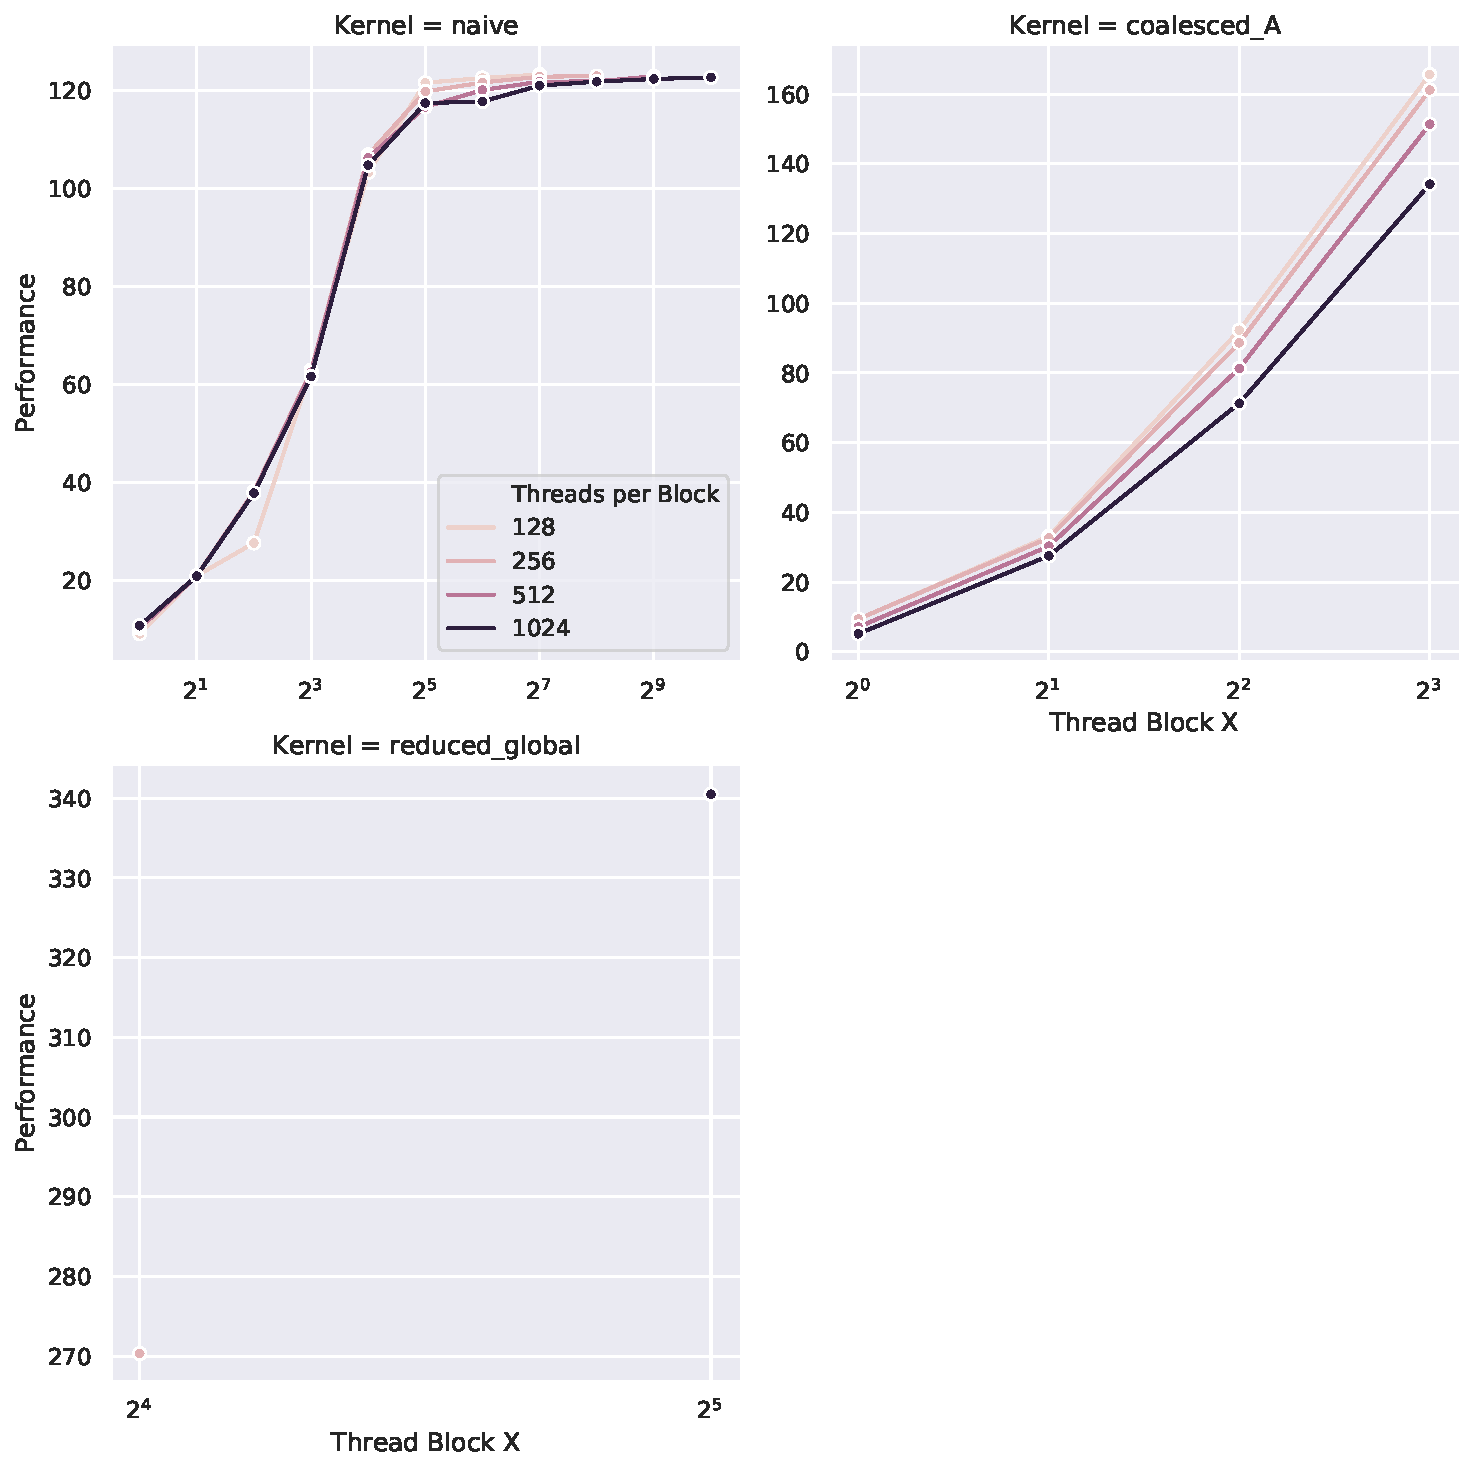
\includegraphics[width=\textwidth]{z1.pdf}
    \selectlanguage{greek}\caption{}
\end{figure}

Ξεκινάμε με την αφελή υλοποίηση που δε χρησιμοποιεί κοινή μνήμη. Επομένως αναζητούμε τις βέλτιστες τιμές για τις διαστάσεις των blocks. Δοκιμάζουμε όλες τις δυνάμεις του 2 εντός των επιτρεπτών ορίων (από 1 έως 1024) για το THREAD\_BLOCK\_X και θέτουμε το THREAD\_BLOCK\_Y έτσι, ώστε τα συνολικά νήματα ανά block να είναι 128, 256, 512 ή 1024 (οι τιμές για τις οποίες μάθαμε ότι μεγιστοποιείται το occupancy). Τα αποτελέσματα φαίνονται στο σχήμα 1.

Εμφανώς η επίδοση είναι πρακτικά ίδια για όλα τα πλήθη νημάτων ανά block. Αυτό που φαίνεται να είναι πολύ σημαντικό ωστόσο είναι το THREAD\_BLOCK\_X να είναι τουλάχιστον 32 (ύστερα η αύξηση της επίδοσης είναι σχετικά ασήμαντη). Το αποτέλεσμα εξηγείται αν αναλογιστούμε ότι το THREAD\_BLOCK\_X καθορίζει το πλήθος των στοιχείων του δεξιού πίνακα που θα προσπελάσουν τα νήματα ενός block σε μια επανάληψη του εσωτερικού βρόχου. Καθώς η προσβάσεις σε αυτό τον πίνακα μπορούν να συνενωθούν, θέλουμε να εκτελούνται τουλάχιστον 32 προσβάσεις, ήτοι ένα ολόκληρο warp να εκτελεί μια μοναδική δοσοληψία με την κύρια μνήμη. Έτσι καταφέρνουμε να μειώσουμε αισθητά την ποινή που επιβάλλει η πρόσβαση στην κυρία μνήμη.

Προχωράμε στην υλοποίηση που φέρνει τον αριστερό πίνακα στην κοινή μνήμη. Εδώ δοκιμάζουμε τις τιμές για τις οποίες λάβαμε occupancy 100\% προηγουμένως. Προκύπτουν τα αποτελέσματα του σχήματος 1. Βλέπουμε εύκολα ότι η αύξηση του THREAD\_BLOCK\_X οδηγεί σε σημαντική αύξηση της επίδοσης. Μεταξύ των διαφόρων τιμών για το πλήθος των νημάτων ανά block υπάρχει σχετικά μικρή αλλαγή στην επίδοση. Ωστόσο φαίνεται οι μικρότερες τιμές να έχουν ένα μικρό προβάδισμα.

Τέλος για την υλοποίηση που φέρνει αμφότερους τους πίνακες στην κοινή μνήμη δοκιμάζουμε τις 2 τιμές που υπολογίσαμε προηγουμένως (πάλι αυτές που μας έδωσαν πλήρες occupancy). Τα αποτελέσματα παρατίθενται στο σχήμα 1. Εύκολα βλέπουμε ότι το 32 σαφώς υπερτερεί του 16. Αυτό είναι λογικό, καθώς σημαίνει πως μπορούμε να αποθηκεύσουμε με λιγότερες δοσοληψίες τα δεδομένα μας στην κοινή μνήμη. Υπερτερεί επομένως η λύση με τη μέγιστη κοινή μνήμη (αρκεί να μην αρχίσουμε να θυσιάζουμε σε occupancy).

Πλέον έχουμε καθορίσει τις βέλτιστες τιμές για τις παραμέτρους μας, οπότε είμαστε σε θέση να συγκρίνουμε τους πυρήνες μας μεταξύ τους για διάφορες τιμές των διαστάσεων. Χάριν ευκολίας στην απεικόνιση προτιμούμε να παραστήσουμε την επίδοση ως προς το γινόμενο των διαστάσεων (αντί για κάθε διάσταση χωριστά). Στην ουσία παραδεχόμαστε ότι μας ενδιαφέρει περισσότερο το συνολικό μέγεθος των πινάκων, παρά οι διαστάσεις καθαυτές. Η παραδοχή μας φαίνεται να ισχύει ικανοποιητικά τουλάχιστον για τους 2 πυρήνες που έχουν συνενώσει και τις προσβάσεις του αριστερού πίνακα στην κύρια μνήμη.

\begin{figure}[h!]
    \begin{subfigure}{0.49\textwidth}
        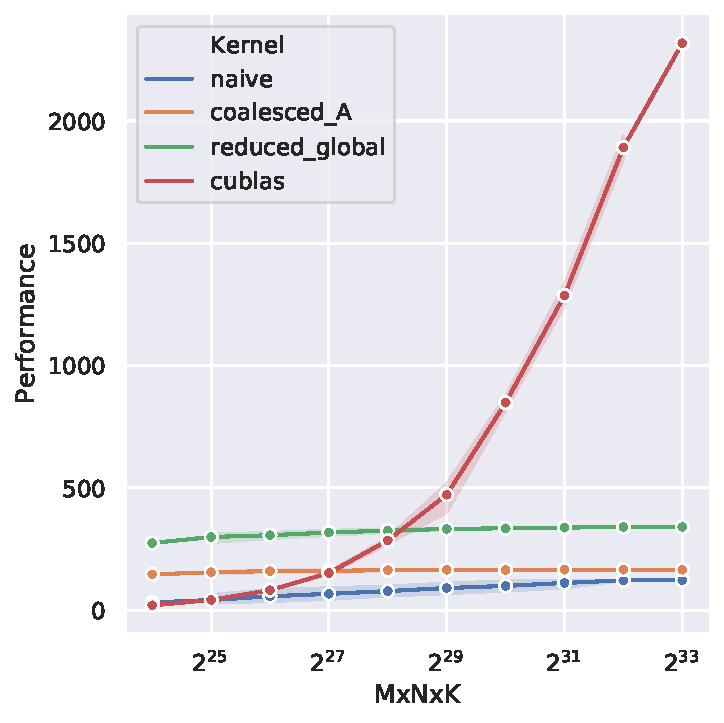
\includegraphics[width=\textwidth]{z2_cublas.pdf}
        \caption{}
    \end{subfigure}
    \begin{subfigure}{0.49\textwidth}
        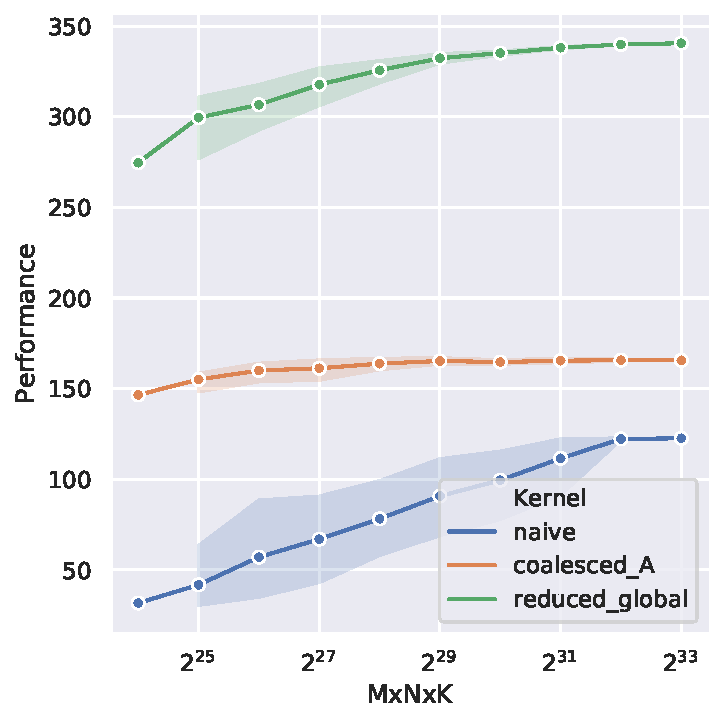
\includegraphics[width=\textwidth]{z2.pdf}
        \caption{}
    \end{subfigure}
    \selectlanguage{greek}\caption{}
\end{figure}

Επιπλέον παραθέτουμε μια φορά όλα τα αποτελέσματά μας συγκεντρωμένα (σχήμα 2α) και μια φορά χωρίς τα αποτελέσματα για τη υλοποίηση που χρησιμοποιεί τη βιβλιοθήκη cuBLAS (σχήμα 2β), καθώς είχαν διαφορά τάξης μεγέθους σε σχέση με τα υπόλοιπα (με αποτέλεσμα να καταστρέφουν την εποπτεία).

Αναφορικά με την επίδοση της συνάρτησης της βιβλιοθήκης cuBLAS, βλέπουμε πως για μικρούς πίνακες είναι χειρότερη από την καλύτερη δική μας υλοποίηση. Ωστόσο, για γινόμενο διαστάσεων από 2\textsuperscript{29} και πάνω είναι δραματικά καλύτερη (κλιμακώνει με δραματικά υψηλό ρυθμό). Προφανώς πρόκειται για μια πλέον βελτιστοποιημένη υλοποίηση. Η αποτυχία της για μικρότερους πίνακες πιθανόν οφείλεται στο επιπλέον overhead που εισάγει (λ.χ. σε κάθε κλήση δημιουργούμε και καταστρέφουμε το handle). Βέβαια είναι λογικό η βιβλιοθήκη να ενδιαφέρεται για τη βελτιστοποίηση του πολλαπλασιαμού σε μεγάλους πίνακες (όπου και θα βρίσκει τη μεγαλύτερη εφαρμογή της).

Όσον αφορά τις υπόλοιπες υλοποιήσεις, τα αποτελέσματα είναι τα αναμενόμενα. Βλέπουμε δηλαδή ότι χειρότερη είναι η αφελής, ακολουθεί αυτή που αξιοποιεί την κοινή μνήμη μόνο για τον ένα πίνακα (αυτόν που έχει ανάγκη συνένωσης των αναφορών) και νικήτρια αναδεικνύεται η υλοποίηση που χρησιμοποιεί την κοινή μνήμη για αμφότερους τους πίνακες.

\end{document}
